\chapter{Model of distribution grids}
\label{ch:distrib}
\minitoc

It has long been acknowledged that distribution grids can significantly impact the stability of transmission systems. This is especially true for voltage stability that strongly depends on the behaviour of loads following disturbances~\cite{CutsemBook, kundur}. However, most utilities still use relatively simple load models (\eg compared to generator models) due to the difficulty to gather data on the loads connected to distribution grids~\cite{IndustryLoadModel}.

This difficulty is caused by the fundamentally different nature of transmission and distribution grids. Indeed, a typical transmission grid connects dozens to hundreds of generators for which individual detailed models can be built (\eg during the grid connection request and commissioning phases). Moreover, transmission system operators (TSOs) are also continuously made aware of the state of all generators (connection status, power output, etc.). Distribution grids however supply millions of customers each with their own appliances and behaviour. Therefore, only aggregated models can realistically be derived. The most commonly used load model is the ZIP load (aggregation of a constant impedance, a constant current, and a constant power load) and its derivates whose parameters are usually defined based on surveys and from transmission-level measurements of distribution grid behaviour following disturbances~\cite{IndustryLoadModel}. On top of this, TSOs now represent distributed energy resources (DERs) with aggregate models representative of each generation category (solar, wind) and each connection standard (legacy installations with limited fault ride-through requirements vs.\ modern ones with stricter requirements, small vs.\ large installations).

%, and distribution system operators (DSOs) generally suffer from a lack of observability of their network.

% and their variable nature\footnote{Both the total amount of load and shares of different types of loads (heaters, motors, lamps, etc.) vary with the time of day and the season.}.

With the massive installation of DERs, distribution grids are playing a more and more active role in the stability and security of transmission systems. However, DERs can have a negative impact on system stability as they displace synchronous generation, thereby reducing system inertia and because they tend to disconnect themselves during system disturbances\footnote{This is because, DSOs initially asked for DERs to have very limited fault ride-through capabilities to avoid DERs from feeding faults in the distribution systems. Modern standards require more strict ride-through requirements to avoid large scale disconnection of DERs following a single transmission fault.}. For example, the frequency collapse of Italy in 2003 was partly caused by the unexpected disconnection of 3400~MW of DERs while the frequency was still above 49~Hz~\cite[p115]{Italy2003}. Similarly, DER disconnections also had a significant contribution in the 2019 UK power outage~\cite{2019UKBlackout}. In this case, 150~MW of DER was tripped as a direct consequence of the initial fault (lightning strike caused disconnection of DERs by vector-shift protection). Quickly after, between 350 and 430~MW of DERs were disconnected due to a high rate of change of frequency (RoCoF). At this point, a total of 1500~MW of generation was lost (around 500~MW of which were DERs), exceeding the primary reserve of 1000~MW which ultimately led frequency to drop to 48.8~Hz when under-frequency load shedding (UFLS) was activated. During the event, around 750~MW additional disconnection of DERs occurred due to frequency dropping below 49~Hz (protection of legacy DERs), UFLS activation (tripping entire feeders including DERs), and unknown causes. % On the other hand, there are perspectives regarding the provision of ancillary services by distributed generators.

As discussed in the previous chapters, performing a probabilistic security assessment requires to simulate the grid during severe disturbances and cascading outages. It is thus necessary to adequately model the behaviour of distribution grids during such disturbances and in particular the disconnection of DERs. Simple ZIP models are not able to do this, and more complex models are thus needed. To get better models, section~\ref{sec:distrib_review} reviews the load modelling literature and identifies an adequate modelling methodology. This methodology is then slightly modified in section~\ref{sec:distrib_methodology} and applied to two test cases.

In the first test case (section~\ref{sec:distrib_ISGT}), the methodology is applied on an academic test system to assess the accuracy of the developed load models in the simulation of cascading outages. In the second test case (section~\ref{sec:distrib_CIGRE}), the same methodology is used to study the impact of distribution grids on the transient stability of the Scottish transmission grid. This falls slightly out of scope of the thesis but demonstrates the lack of data issues encountered when modelling real distribution grids. Section~\ref{sec:distrib_conclusion} concludes this chapter with perspectives for future work.


\section{Load modelling review}
\label{sec:distrib_review}

Load modelling generally takes two steps: first, to define a load model, second, to define its parameters. The most commonly-used load models are reviewed in section~\ref{sec:load_models} and the techniques used to estimate their parameters are reviewed in section~\ref{sec:load_parameters}. Section~\ref{sec:distrib_review_conclusion} concludes this review with the techniques available to model distribution grids with large shares of DERs and a discussion of their limitations.


\subsection{Load models}
\label{sec:load_models}

Over the years, many load models have been developed for various studies. This section introduces the most popular ones, and redirects to the reviews of the CIGRE and NERC load modelling task forces~\cite{CIGREloadModels, NERCloadModelTF} for a more comprehensive and detailed review. The earliest and simplest load models were so-called ``static load models''. The behaviour of those loads directly depends on the instantaneous value of voltage and frequency, \ie

\begin{IEEEeqnarray}{rCl}
    P & = & f_P(V, f) \\
    Q & = & f_Q(V, f)
\end{IEEEeqnarray}

This is as opposed to ``dynamic load models'' whose behaviour can also depend on time, the derivatives of voltage and frequency and on their past values.

One of the most commonly-used static load models is the exponential load model whose behaviour is given by

\begin{IEEEeqnarray}{rCl}
    P & = & P_0 \left(\frac{V}{V_0}\right)^\alpha \\
    Q & = & Q_0 \left(\frac{V}{V_0}\right)^\beta
\end{IEEEeqnarray}

The active (resp. reactive) power consumption of this load is thus proportional to the \(\alpha\)th (resp. \(\beta\)th) power of the ratio between the current voltage \(V\) and the initial (or reference) voltage \(V_0\). Particular values of \(\alpha\) and \(\beta\) are 0, 1, and 2 that respectively represent constant-power, constant-current, and constant-impedance loads.

In the 90s to 2010s, more complex load models were developed as some TSOs realised these simple load models did not allow reproducing historical blackouts in post-mortem analysis. The main element that was then added in load models was the induction motor. Indeed, induction motors represent a large share of load especially in industrialised countries and in regions with a lot of air conditioning. And these motors can have a large impact on voltage stability and small-signal stability. A simple load model including an induction motor is shown in Figure~\ref{fig:motorLoad}. This model consists of a constant-impedance load in parallel with an induction motor. The slip \(s\) of the motor is modelled with a classical swing equation.

\begin{IEEEeqnarray}{rCl}
    s & = & \frac{\omega_{ref} - \omega}{\omega_{ref}} \\
    2 H \frac{d\omega}{dt} & = & c_e - c_l
\end{IEEEeqnarray}
\noindent where \(\omega\) is the angular speed of the motor and \(\omega_{ref}\) the angular speed of the grid, \(H\) is the inertia of the motor, and \(c_e\) and \(c_l\) are the electrical and load torques of the motor.

\begin{figure}
    \centering
    \includegraphics[width=0.6\linewidth]{Figs/MotorLoad.png}
    \caption{Constant impedance load in parallel with an induction motor~\cite{CIGREloadModels}}
    \label{fig:motorLoad}
\end{figure}

More complex load models have also been developed such as the WECC composite load model (CLM) shown in Figure~\ref{fig:WECC-CLM}. This model consists of a static (ZIP) load in parallel with 4 different types of induction motors and an electronic load, all behind an equivalent feeder impedance. The electronic load is a constant power load that can (partly) disconnect after severe voltage drops. The feeder model also includes an on-load tap changer to regulate distribution voltage on the long-term.

\begin{figure}
    \centering
    \includegraphics[width=0.5\linewidth]{Figs/WECC-composite-load-model.png}
    \caption{WECC composite load model~\cite{NERCloadModelTF}}
    \label{fig:WECC-CLM}
\end{figure}

The models presented above however do not consider distributed energy sources, and so, even more complex models have recently been developed. This is usually done by adding a DER model to an existing load model. For example, EPRI has developed a DER model called der\_a and recommends adding it to the WECC CML, at the end of the feeder (\eg to represent rooftop solar) and/or at the start (\eg to represent distribution-connected wind farms).

A large share of DERs consists of solar and wind generation, \ie inverter-based generation. DERs are thus often represented with generic models as shown in Figure~\ref{fig:IBG}. These models represent (grid following) inverter-based generation as current-controlled sources with the following control blocks.

\begin{figure}
    \centering
    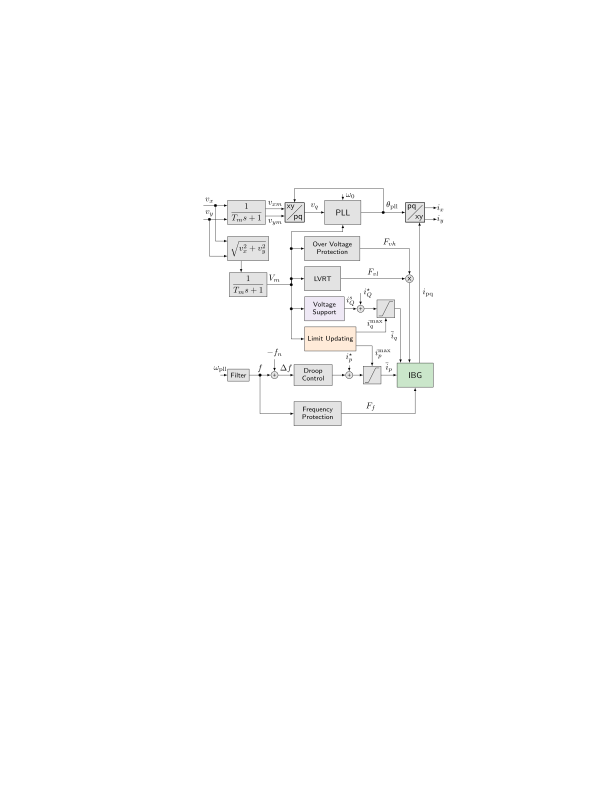
\includegraphics[width=0.6\linewidth]{Figs/IBG.pdf}
    \caption{Generic model of inverter-based generation, based on~\cite{Vorwerk}}
    \label{fig:IBG}
\end{figure}

\begin{itemize}
    \item Current limiter (Limit Updating) that limit the active and reactive current commands (\(i_P\) and \(i_Q\)) to keep the total current (\(\sqrt{i_P^2 + i_Q^2}\)) within the inverter ratings.
    \item Grid support blocks (Voltage support, Droop control) that help with voltage and frequency stability. These functions are usually not present in legacy inverters but are requested by recent grid codes (\eg~\cite{G99}).
    \item Protection blocks (Over-Voltage Protection, Low-voltage ride-through (LVRT), Frequency Protections) that disconnect DERs during large disturbances. As DER model are used to represent many individual generators, it is necessary to account for the fact that only part of the generators might trip (legacy inverters being more likely to trip than recent ones). These blocks thus multiply the current commands by factors between 0 and 1 (0 represent a complete trip of all generators, and 1, no trips).
    \item A phase-locked loop (PLL) and inverter model (IBG) to transform the active and reactive current commands to actual currents.
\end{itemize}

% One way to accurately model the interactions between the transmission and distribution sides of a grid is to perform simulations on complete a transmission and distribution network as in~\cite{FullTDexample}\footnote{To limit the size of the studied system, it is of course necessary to only consider the medium voltage level of the distribution grids, not the low voltage level.}. However, this approach cannot be used in this thesis due to the high computational power requirements of probabilistic dynamic security assessment. Outside the scope of this thesis, this approach also has issues of confidentiality and data handling.



\subsection{Estimating the parameters of load models}
\label{sec:load_parameters}

A model is only complete once numerical values have been assigned to its parameters. However, estimating the parameters that give the most accurate representation of the system might be difficult, especially since TSOs have little observability on distribution grids.


% \usepackage[edges]{forest}
% \begin{forest}
%     forked edges,
%     for tree={grow=south,draw,
%     font=\strut\footnotesize\sffamily\em},
%     [Load modelling
%         [Component-based approach]
%         [Parameter fitting
%             [Measurement-based]
%             [Simulation-based]]
%     ]
% \end{forest}

Two main types of methods exist to estimate the best parameters for load models: the component-based approach, and the parameter identification approach.

In the component-based approach, surveys, billing data and other data are used to estimate what is the share of the total load that is consumed by different types of loads. Commonly, loads are classified in residential, commercial, industrial, and agricultural loads. More refined classifications can also be used, for example, splitting industrial loads in petrochemical, mining, smelting, etc. Based on lab testing and validation with historical disturbances, parameters can be estimated for each of these load types. For example, when using the WECC CLM, NERC recommends modelling steel mills as loads with a 75\% motor share, a 20\% power electronic share, and a 5\% static load share. For server farms, it is instead 40\% of motors, and 60\% of power electronics~\cite{component_based}. The final parameters of the total load are then computed using weighted averages of the parameters of the various load subtypes. It should be noted that, as this process is quite complex (estimation of the share of different load types that vary with the time of day, and estimation of the load parameters for each load subtype), some form of sensitivity analysis should be performed to see how modelling uncertainties in load models affect the results of system studies.

In the parameter identification approach, the parameters of the load models are tuned such that the model behaves as closely as possible to some reference for a given set of disturbances. Mathematically speaking, this means finding the vector of parameters \(\bm{\theta}\) that minimises some sort of sum of square error between the behaviour of the load model and the behaviour of the reference as in the example formulation below.

\begin{IEEEeqnarray}{rCl}
\min_{\bm{\theta}} F(\bm{\theta}) & = & \frac{1}{d} \sum_{j=1}^d \left[F_P(\bm{\theta}, j) + F_Q(\bm{\theta}, j)\right] \\
%
\text{with } F_P(\bm{\theta}, j) & = &  \frac{1}{T} \sum_{t=1}^T \left[P(\bm{\theta}, j, t) - \hat{P}(j, t)\right]^2\\
%
F_Q(\bm{\theta}, j) & = &  \frac{1}{T} \sum_{t=1}^T \left[Q(\bm{\theta}, j, t) - \hat{Q}(j, t)\right]^2\\
%
\bm{\theta}^L \leq \bm{\theta} & \leq & \bm{\theta}^U
\end{IEEEeqnarray}
%
\noindent where \(P(\bm{\theta}, j, t)\) (resp. \(Q(\bm{\theta}, j, t)\)) is the active (resp. reactive) power consumed by the load model \(t\) time steps (out of \(T\)) after the occurrence of disturbance \(j\), and \(\hat{P}(j, t)\) (resp. \(\hat{Q}(j, t)\)) is the active (resp. reactive) power consumed by the reference at the same time and for the same disturbance. \(\bm{\theta^L}\) and \(\bm{\theta^U}\) are lower and upper bounds on the parameters of the load models used to guarantee that the load models get realistic values.

The reference can either be time-series of measurements obtained after actual disturbances (measurement-based approach) or from detailed simulations (simulation-based approach). The measurement-based approach has the potential to give very accurate models as it is directly based on real measurements of the load behaviour. However, large disturbances are fortunately rare, so it might be difficult to obtain measurements for a sufficiently representative set of disturbances. Moreover, models obtained this way are only valid for one snapshot in time for which the measurement event occurred. The amount of PV disconnections will significantly vary between day and night times for example. Measurement-based approaches are thus mostly useful to validate the models obtained with other approaches\footnote{For small disturbances, developing models purely based on measurements is appropriate as small disturbances are more common and can be artificially created with transformer tap changes.} (the importance of model validation should however not be neglected).

In simulation-based approaches, distribution grids are simulated for a wide range of disturbances using a ``full model''. The results of these simulations are then used as a reference to tune the parameters of the load model (also called reduced model or dynamic equivalent). The challenge then becomes the definition of an appropriate full model. In many academic works, it has simply been assumed that such full model would be available~\cite{fulgencio}, \ie that DSOs would have detailed dynamic models of their networks which appears to us as unrealistic.

In~\cite{ChaspierrePaper, ChaspierreThesis} however, this assumption has been strongly relaxed and authors assumed that only static data (\ie branch impedances and resistances) would be available. For dynamic data, generic models were used for motors and DERs. The parameters of those dynamic models were assigned (relatively wide) probability density functions based on expert knowledge. Monte Carlo (MC) simulations were then performed to evaluate the impact of those uncertain dynamic parameters on the behaviour of loads. Finally, the parameters of the dynamic equivalents were fitted to match either the average behaviour of the uncertain full model. This is illustrated in Figure~\ref{fig:VDrop6}. In this figure, dotted lines show the results of MC simulations of a full distribution model following a voltage drop. From these simulations, the average behaviour can be estimated (brown full line), and the parameters of an equivalent can be fitted to match this average (brown dotted lines)\footnote{The MC simulations shown in Figure~\ref{fig:VDrop6} seem to aggregate around 2 main clusters: one with no or little trips of DERs (net load recovers to pre-fault values) and one with significant trips. This begs the question of why not clustering the results of MC simulations (\eg using K-means) and building one equivalent per cluster. Some tests were performed in this direction, however, once multiple disturbances are considered, the separation between clusters becomes less obvious. Cluster centroids are then likely to miss extreme cases. The percentile-based approach is much more robust in this regard.}.

However, Figure~\ref{fig:VDrop6} also shows that, due to high uncertainty, the actual load behaviour might strongly differ from the average expected behaviour. Building equivalents based on quantiles instead of averages might thus be more appropriate.

In~\cite{Vorwerk}, authors also used MC simulations to assess the impact of uncertainties of load behaviour. They then used machine-learning-based quantile forecasting to build an interval of potential load behaviour in addition to the mean behaviour. However, they only considered mild disturbances (load steps, not faults) and did not test their load model in transmission studies. Also, the final load model in~\cite{Vorwerk} is not a physical model but an artificial neural network whose behaviour is harder to interpret.

\begin{figure}
\centering
\begin{tikzpicture}
\pgfplotsset{width=0.7\linewidth}
\begin{axis}[
    xlabel={Time [s]},
    xmin=0, xmax=5,
    ylabel= {P [MW]},
    legend cell align=left,
    legend style={at={(1,0)},anchor=south east},
    ]

    \foreach \n in {0,...,49}{
        \addplot+ [mark=none, color=black, dotted, opacity=0.7, line width=0.6pt] table [x=time,y=VDrop6_\n] {Figs/VDrop6.txt};
    }
    \addplot+ [mark=none, line width=1pt, blue] table [x=time,y=Percentile5] {Figs/VDrop6Percentiles.txt};
    \addplot+ [mark=none, dashed, line width=1pt, blue] table [x=time,y=VDrop6] {Figs/VDrop6_5Fit.txt};
    \addplot+ [mark=none, line width=1pt, red] table [x=time,y=Percentile95] {Figs/VDrop6Percentiles.txt};
    \addplot+ [mark=none, dashed, line width=1pt, red] table [x=time,y=VDrop6] {Figs/VDrop6_95Fit.txt};
    \addplot+ [mark=none, line width=1pt, brown] table [x=time,y=VDrop6] {Figs/VDrop6_average.txt};
    \addplot+ [mark=none, dashed, line width=1pt, brown] table [x=time,y=VDrop6] {Figs/VDrop6_average_fit.txt}; % Actually this is the average of fit_5 and fit_95 because I don't want to resimulate it
    % \addlegendentry{Percentile 5}
    % \addlegendentry{Percentile 95}
    % \addlegendentry{Average}
    % \addlegendentry{5-equivalent}
    % \addlegendentry{95-equivalent}
    % \addlegendentry{MC samples}
    \legend{,,,,,,,,,,,,,,,,,,,,,,,,,,,,,,,,,,,,,,,,,,,,,,,,, MC samples,Percentile 5, 5-equivalent, Percentile 95, 95-equivalent, Average, Average equivalent}

\end{axis}
\end{tikzpicture}
\caption{Behaviour of the reduced (dashed lines) and unreduced (dotted and full lines) models of a distribution grid following a temporary voltage drop (disturbance 6 of Table~\ref{tab:disturbances}). The net load drawn after the drop is increased mainly due to disconnection of DERs (in uncertain amount).}
\label{fig:VDrop6}
\end{figure}

% \item Black-box approaches: in these methods, the model of a distribution system is an artificial neural network (ANN) that is trained to match the behaviour of the actual distribution system. These methods are quite popular since they do not require any information on the structure and components of the distribution grid. ANNs are thus most often matched to measurements of the behaviour of the distribution grid (often PMU measurements made at the point of common coupling (PCC) between the transmission and distribution grids). It is also possible to train ANNs from simulations of the distribution grid, but grey-box approaches (described below) are often preferred when one has enough information on the distribution grid to simulate it. The main limitation of measurement-based approaches (and by extension black-box approaches) is that large disturbances are rare. It is possible to intentionally introduce disturbances to generate more data but those disturbances are usually kept small for obvious reasons (usually tap changes or capacitor switching). Training ANNs for those disturbances is thus often impossible.
% \item Grey-box approaches: grey-box approaches are similar to black-box approaches except that the model used is a physical model instead of an ANN. The model usually has at most a few buses and should have a similar structure than the real grid\footnote{Taking the example shown in Figure~\ref{fig:greyBox}, if switches a and b are closed, and switch c is open, they grey-box model becomes two feeders in parallel. One feeder could represent a classical distribution system. The second, a large distribution-connected plant (with stricter connection requirements).}. The advantage is thus that results are more comprehensive, but it is necessary to known  the structure of the distribution grid. An example of grey-box model is shown in Figure~\ref{fig:greyBox}. Like black-box approaches, the parameters of the model are fitted to match the behaviour of the full model (\eg in the least square sense). As it is not feasible to write the analytical formulation of the objective function (\ie difference between behaviour of the grey-box and the real system), derivative-free optimisation methods (\eg genetic algorithms, particle swarm optimisation) have to be used. The behaviour of the real system for a given operating point and disturbance can be obtained either from measurements or from simulations. As previously explained, only the simulation-based approach is appropriate when studying large disturbances\footnote{When available, measurements should still be used to validate the equivalent and/or the full distribution model.}.

    % \item Linear-based approaches: in these methods, the model of the full distribution network is first linearised. Then, different approaches (\eg Hankel-norm approximation, modal approach, Krylov methods, etc.) allow to reduce the order of the linearised system. A theoretical bound on the error made by using the reduced-order model can be derived depending on the method used. These methods are however accurate only around a given operating point and are thus not appropriate to study large disturbances. These methods were originally developed to make reduced-order equivalents of neighbouring transmission systems. Indeed, TSOs mostly study the impact of disturbances originating in their own system. For moderately large disturbances, neighbouring TSOs are weakly affected, so a linearisation-based approach makes sense. Distribution systems however are much more dependent on their associated transmission system.
    % \item Coherency-based approaches: synchronous generators that tend to swing together are grouped into an equivalent machine. The network around those machines is then also reduced. Like linear-based approaches, these methods were developed to model neighbour transmission systems. They are often not applicable to distribution systems as synchronous generators are rarely used there.

% \begin{figure}
%     \centering
%     \includegraphics[width=0.6\linewidth]{Figs/GreyBoxEquivalent.pdf}
%     \caption{Possible grey-box equivalent topologies. Multiple topologies can be created from this scheme by changing the status of the switches~\cite{ChaspierreThesis}. IBG = Inverter-based generation}
%     \label{fig:greyBox}
% \end{figure}



\subsection{Conclusion}
\label{sec:distrib_review_conclusion}

This section reviewed three main approaches for load modelling (the component-based approach, the measurement-based approach, and the simulation-based approach) and discussed their advantages and limitations for simulating large disturbances. The component-based approach is the most popular amongst TSOs. However, it is rather involved, requiring to model potentially many types of loads and to estimate their shares in the total load. Moreover, it does not provide a direct way to perform sensitivity studies which are needed to validate the obtained load models.

The measurement-based approach is limited by the fact that large disturbances are rare. It should therefore be avoided when building load models from scratch. However, real measurements should definitively be used to validate the models obtained with other methods.

The main advantage of the simulation-based approach (at least the variants proposed in~\cite{ChaspierreThesis, ChaspierrePaper, Vorwerk}) is that it allows to easily perform sensitivity studies. This is generally important due to the complexity in developing adequate load models, but is even more important in the context of probabilistic security assessment. Indeed, probabilistic security assessments require simulating the system during cascading outages and very degraded states which challenges the accuracy of the (load) models used. The simulation-based approach is thus used in this thesis.

Section~\ref{sec:distrib_methodology} presents the load modelling methodology used in this thesis. As the methodology of~\cite{ChaspierreThesis, ChaspierrePaper} is quite powerful, it is used as strong basis for this work. The main difference is that this thesis uses percentiles instead of the average expected load behaviour.

Also, \cite{ChaspierreThesis, ChaspierrePaper} developed their models to study voltage stability issues and thus did not test their models for the simulation of cascading outages. And generally speaking, the majority of the literature on cascading outage simulation uses simple load models. Section~\ref{sec:distrib_ISGT} thus applies the methodology to the simulation of cascading outages on a standard test system.

% \begin{figure}
%     \centering
%     \includegraphics[width=0.6\linewidth]{Figs/GreyBoxUncertainty.png}
%     \caption{Average \(\mu_P\) and standard deviation \(\sigma_P\) of the active power consumption of a distribution grid following a disturbance at \(t=\)0.3~s~\cite[p58]{ChaspierreThesis}}
%     \label{fig:greyBoxUncertainty}
% \end{figure}


\section{Proposed load modelling approach}
\label{sec:distrib_methodology}

As stated, the methodology used in this thesis is strongly based on the one proposed in~\cite{ChaspierrePaper, ChaspierreThesis}. The methodology consists in two main parts. In the first part, a detailed model of the considered distribution grid is built. As modelling distribution grids is very complex, the parameters of the detailed model will be assigned very wide (and usually uniform) probability density functions based on expert knowledge (giving lower and higher realistic bounds for all parameters). MC simulations are then performed on a set of \(d\) disturbances to evaluate the impact of the uncertain modelling of the distribution grid on its behaviour.

Of particular interest are the active and reactive power at the point of common coupling (PCC) with the transmission grid. Thus, the following values are extracted from the MC simulations: \(\mathscr{P}_{P, i}(j, t)\) (resp. \(\mathscr{P}_{Q, i}(j, t)\)), the \(i\)th percentile over all MC simulations of the active (resp. reactive) power drawn during the \(j\)th disturbance at time \(t\); and \(\sigma_P(j,t)\) (resp. \(\sigma_Q(j,t)\)), the standard deviation of the active (resp. reactive) power for the same disturbance and at the same time.

In the second part, two dynamic equivalents of the distribution system model are built to bound the uncertain behaviour of the distribution grid: one (referred to as the 5-equivalent) that fits the 5th percentile of the active and reactive power of the distribution system, and one that fits the 95th percentile as shown in Fig.~\ref{fig:VDrop6}. Mathematically, the vector of parameters \(\bm{\theta}\) of each dynamic equivalent is taken as the solution of the following weighted least-square optimisation problem:

\begin{IEEEeqnarray}{rCl}
\label{eq:equivalent_optimisation}
\min_{\bm{\theta}} F(\bm{\theta}) & = & \frac{1}{d} \sum_{j=1}^d \left[F_P(\bm{\theta}, j) + F_Q(\bm{\theta}, j)\right] \\
%
\text{with } F_P(\bm{\theta}, j) & = &  \frac{1}{T} \sum_{t=1}^T \left[\delta_{i, P, j, t} \frac{P(\bm{\theta}, j, t) - \mathscr{P}_{P, i}(j, t)}{\sigma_P(j,t)}\right]^2\\
%
F_Q(\bm{\theta}, j) & = &  \frac{1}{T} \sum_{t=1}^T \left[\delta_{i, Q, j, t} \frac{Q(\bm{\theta}, j, t) - \mathscr{P}_{Q, i}(j, t)}{\sigma_Q(j,t)}\right]^2\\
%
\bm{\theta}^L \leq \bm{\theta} & \leq & \bm{\theta}^U
\end{IEEEeqnarray}
\noindent with \(i\) equal to 5 or 95. This formulation differs from the one in~\cite{ChaspierrePaper, ChaspierreThesis} only by the use of percentiles instead of the average behaviour. Also, the term \(\delta_{i, P, j, t}\) is added and is defined by

\begin{equation}
\delta_{5, P, j, t} = \left\{\begin{array}{lr}
    1 & \text{if } P(\bm{\theta}, j, t) \leq \mathscr{P}_{P, 5}(j, t) \\
    \frac{1}{2} & \text{if } P(\bm{\theta}, j, t) > \mathscr{P}_{P, 5}(j, t)
    \end{array}\right.
\end{equation}
\begin{equation}
\delta_{95, P, j, t} = \left\{\begin{array}{lr}
    1 & \text{if } P(\bm{\theta}, j, t) > \mathscr{P}_{P, 95}(j, t) \\
    \frac{1}{2} & \text{if } P(\bm{\theta}, j, t) \leq \mathscr{P}_{P, 95}(j, t)
    \end{array}\right.
\end{equation}

The term \(\delta_{i, Q, j, t}\) has a similar definition. This factor results in a lower penalty for the equivalent that fits the 95th percentile if it consumes too much power (compared to the 95th percentile) and in a lower penalty for the 5-equivalent if it consumes too little. This leads to more conservative bounds on the behaviour of the distribution system. The main reason for adding this factor is that otherwise the numerical solution of the optimisation problem tends to converge to a solution that is closer to the average behaviour than expected. This is because it is usually easier to find a set of parameters to matches the average behaviour of the load model than its extremes.

Also, it should be noted that percentiles are computed individually for each disturbance and each point in time. Those percentiles are thus synthetic and represent an envelope of the possible behaviours of the distribution grid, not a likely behaviour which also makes it more complicated to find an optimal value for \(\bm{\theta}\).

Speaking of numerical solution, there is no analytical formulation of \(P(\bm{\theta}, j, t)\) and its derivatives are difficult to estimate. A derivative-free approach is thus necessary to solve the optimisation problem. The differential evolution (DE) algorithm was used in~\cite{ChaspierreThesis, ChaspierrePaper} and is thus also used in this thesis. As it showed good performance, no other technique has been tested in this thesis. As in~\cite{ChaspierreThesis, ChaspierrePaper}, DE is stopped once sufficient accuracy is reached, \eg when

\begin{equation}
    \label{eq:equivalent_stop}
    F_P(\bm{\theta}, j) \leq 1 \text{ and } F_Q(\bm{\theta}, j) \leq 1
\end{equation}

\noindent \ie when the behaviour of the equivalent is on average less than one standard deviation away from the behaviour of the full model.

It should be noted that, \cite{ChaspierreThesis} developed a methodology to update the parameters of the load model when operating conditions change (\eg if solar irradiation increases, the behaviour of the load will change as well as its parameters). However, for the sake of simplicity, load models were always parametrised from scratch in the test cases in this chapter.

% In~\cite{ChaspierreThesis}, a Least Absolute Shrinkage and Selection Operator (LASSO) was used in complement to DE in order to identify the parameters of the equivalent which are the most significant. This led to slow convergence in our case as more parameters deviate from their average value when fitting a 5th or 95th percentile than when fitting an average. If one wants to identify significant parameters, some form of sensitivity analysis might be more efficient.

% He also proposed a methodology to share the grey-box development between the TSO and DSOs to avoid confidentiality issues, and he discussed how to efficiently update the equivalent with varying operating conditions. Interestingly, he also proposed a control algorithm for a battery storage to be installed at the PCC to compensate for errors between the grey-box and the real system. Those elements are however not discussed further here.


It is common to ``train'' an equivalent by connecting it to an infinite bus to which voltage (and possibly angle and frequency) disturbances are applied~\cite{ChaspierreThesis, CIGREloadModels, fulgencio}. However, in this thesis, it was found that connecting it to a synchronous machine that has the same rating as the total gross load through a line with an impedance of 0.1~pu leads to equivalents which are more accurate in transmission studies. This is because it allows for easier incorporation of fault-induced delayed voltage recovery events into the training set of the equivalent. Also, it makes \(P(\bm{\theta}, j, t)\) more sensitive to \(\bm{\theta}\). This is further discussed in section~\ref{sec:isgt_results_visual}.

It should be noted that the synchronous machine and line do not aim to be an equivalent of the transmission system as seen from the distribution system. As will be shown in section~\ref{sec:distrib_ISGT}, equivalents built this way have a very good accuracy even when used at different locations with different system strengths, and during cascading outages during which the system strength at a given location can significantly vary\footnote{Other modifications were made compared to~\cite{ChaspierreThesis} in order to help the convergence of DE and are listed below. However, additional tests should be performed to validate the relevance of those modifications.
\begin{itemize}
    \item \cite{ChaspierreThesis} uses a least absolute shrinkage and selection operator (LASSO) to identify the most important parameters of the equivalents. This works by adding a penalty to the objective function when identified parameters deviate from their expected value (average of \(\bm{\theta}^L\) and \(\bm{\theta}^U\)), and decreasing the penalty until a solution that satisfies (\ref{eq:equivalent_stop}) is found. This works well for the average equivalent, but for the 5- and 95-equivalents, many parameters deviate from their expected value which slows down convergence and requires to use a small penalty term. Most parameters are then identified as critical by the LASSO.
    \item \cite{ChaspierreThesis} iteratively added disturbances to (\ref{eq:equivalent_optimisation}), stopping early if the equivalent trained with a small set of disturbances was valid (\ie satisfied (\ref{eq:equivalent_stop})) for all disturbances. In this work however, it was necessary to train using many disturbances to correctly fit the tripping parameters, so it was faster to directly train the equivalent with all considered disturbances.
\end{itemize}
}.


The training disturbances used in this work are impedant short-circuits of different durations applied at the PCC, leading to more or less severe voltage drops as listed in Table~\ref{tab:disturbances}. More or less impedant short-circuit represent faults that are more or less far away from the load. Additionally, if the equivalent is to be used in a case where the frequency goes outside the [49, 51]~Hz range (cascading outages), frequency ramps are added to the training disturbances to fit the frequency related parameters of the equivalent. Four ramps are considered here, going respectively from 50~Hz to 47.5, 48.5, 51.5, and 52.5~Hz, all in 1.5s.

\begin{table}
\centering
\caption{Training disturbances}
\label{tab:disturbances}
\begin{tabular}{@{}ccc@{}}
\toprule
ID & Voltage dip (pu) & Duration (ms) \\ \midrule
1  & 0.2               & 100           \\
2  & 0.2               & 200           \\
3  & 0.3               & 100           \\
4  & 0.3               & 200           \\
5  & 0.4               & 100           \\
6  & 0.4               & 200           \\
7  & 0.5               & 100           \\ \bottomrule
\end{tabular}
% \hfill
\hspace{1cm}
\begin{tabular}{@{}ccc@{}}
\toprule
ID & Voltage dip (pu) & Duration (ms) \\ \midrule
8  & 0.5               & 200           \\
9  & 0.7               & 100           \\
10 & 0.7               & 200           \\
11 & 0.8               & 200           \\
12 & 0.8               & 500           \\
13 & 0.9               & 500           \\
14 & 0.9               & 1000          \\ \bottomrule
\end{tabular}
\end{table}


\section{Test case 1: Simulation of cascading outages}
\label{sec:distrib_ISGT}

\begin{tcolorbox}[width=\linewidth, sharp corners=all,
    colback=white!80!black,
    colframe=white!80!black]
This section is partly based on the following publication:
\begin{itemize}
    \item \fullcite{ISGT2023_ADN}
\end{itemize}
\end{tcolorbox}


The objective of this test case is to study if the dynamic equivalencing methodology proposed in section~\ref{sec:distrib_methodology} is adequate to study cascading outages. To do this, simulations of cascading outages will first be performed on a complete model of an academic transmission and distribution system (\ie complete grid model from 400~kV to 20~kV), then the same simulations will be performed but replacing the distribution grid models by simpler equivalents. The distribution grid models used in this test case are described in section~\ref{sec:isgt_distrib} and the complete transmission and distribution grid model is described in section~\ref{sec:isgt_TD}. The simulation results obtained with the full and reduced distribution models are compared in section~\ref{sec:isgt_results}.

\subsection{Distribution system}
\label{sec:isgt_distrib}

The distribution system considered in this test case is based on the CIGRE medium voltage (MV) network\footnote{Static data is available for this network. However, the methodology is very generic and could still be applied if the static data was uncertain. This is performed in the second test case (section~\ref{sec:distrib_CIGRE})}~\cite{CIGREMV} shown in Figure~\ref{fig:CIGRE_MV}. Loads 1 and 12 (that account for almost 90\% of the total load) have been removed as they represent separate feeders and do not include data on DERs. The distribution transformers have been downscaled to match the original voltage profile. Finally, the PV and wind installations have been upscaled to reach each 40\% of the total load. Results presented in this section were obtained at an operating point with 100\% wind availability and 25\% solar availability, leading to an instantaneous inverter-based generation (IBG) penetration of 50\%.


\begin{figure}
\centering
\subfloat[CIGRE MV network with solar and wind generation~\cite{CIGREMV}]{%
    \includegraphics[width=0.6\linewidth]{Figs/cigre_network_mv.png}
    \label{fig:CIGRE_MV}
    } \hfill
\subfloat[Dynamic equivalent]{%
    \begin{tikzpicture}[scale = 0.8, transform shape]

    \draw [line width=0.7mm](6,1.5) -- (8,1.5);
    \draw (7,2.5) node[gridnode](extgrid){};
    \draw (7,2) to [short] (7,1.5);

    \draw (7,1.5) to [oosourcetrans] (7,0);
    \draw [line width=0.7mm](6,0) -- (8,0);
    \draw (7,0) to [short] (7,-2);
    \draw [line width=0.7mm](5,-2) -- (10,-2);

    \draw [-{Latex[scale=0.7]}] (6.5,0) -- (6.5,-0.4);
    \draw [-{Latex[scale=3]}] (5.5,-2) -- (5.5,-4);
    \draw (6.5,-3.5) node[elmech](M1){M};
    \draw (7.5,-3.5) node[elmech](M1){M};
    \draw (6.5,-3) to [short] (6.5,-2);
    \draw (7.5,-3) to [short] (7.5,-2);

    \draw (8.1,-3.8) rectangle (8.9,-3.2) node[midway] {IBG};
    \draw (9.1,-3.8) rectangle (9.9,-3.2) node[midway] {IBG};
    \draw (8.5,-3.2) to [short] (8.5,-2);
    \draw (9.5,-3.2) to [short] (9.5,-2);

    \end{tikzpicture}
    \label{fig:Equivalent}
    }
\caption{Distribution systems used in test case 1}
\label{fig:distrib}
\end{figure}

The dynamic equivalent of the distribution system is a relatively simple model made of one load bus connected to the transmission grid by an equivalent impedance and a distribution transformer as shown in Fig.~\ref{fig:Equivalent}. The load bus consists of an exponential load, two first-order inductor motor models (to allow for stalling of a part of all motors), and two IBG models (one that represents PV units, and one that represents wind).

The IBG model used in the full and reduced distribution models is the one shown in Figure~\ref{fig:IBG} and described in more details in~\cite{ChaspierreThesis}\footnote{The partial tripping models have been slightly modified compared to~\cite{ChaspierreThesis} in order to allow the equivalent model to more accurately fit the behaviour of the distribution system. Please refer to the model implementation available in \url{https://fredericsabot.github.io/Publications.html} for more information.}. The range of uncertain parameters for loads and DERs are given in Table~3.1 in~\cite{ChaspierreThesis}.

\subsection{Transmission \& distribution network}
\label{sec:isgt_TD}

The complete transmission and distribution (T\&D) system considered is built by replacing all loads of the IEEE 39-bus test system (except load 39 which represents an interconnection) by copies of the CIGRE MV network. Each of those copies is scaled such that its gross load is the same as the load it replaces in the 39-bus system. This leads to a reduction of the net load seen on the transmission side (from 6100~MW to 3600~MW) as DERs are now satisfying part of the total load. To account for this, generators 33, 34, and 36 (coal units, so the most expensive) are disconnected and the setpoint of generator 39 is reduced from 1000~MW to 263~MW. To keep the system N-1 secure, a synchronous condenser is added in place of generator 33, and generator 38 is equipped with a faster AVR. The same protection system models (and associated uncertainty) as in section~\ref{sec:protection_test_case} are used.

\subsection{Results}
\label{sec:isgt_results}

The validation of the equivalencing process is made in multiple steps. First, a simple visual comparison of time-domain evolution of the transmission system simulated with full and reduced models of distribution grids is performed as a first intuitive validation and to highlight the importance of correctly training the equivalents. This is performed in section~\ref{sec:isgt_results_visual}. Then, section~\ref{sec:isgt_results_CCT} validates the reduced models for the purpose of a classical transmission system study: the evaluation of generator critical clearing times. Finally, section~\ref{sec:isgt_results_cascading} performs a validation for the actual use case of this thesis: the simulation of cascading outages.


\subsubsection{Visual comparison}
\label{sec:isgt_results_visual}

As stated above, it is common to train equivalents by connecting them to an infinite-bus system to which disturbances are applied. However, this led to inaccurate equivalent models in this thesis. Indeed, Figure~\ref{fig:fault39} shows a significant discrepancy between the voltage evolution at bus 4 following a 100ms fault at bus 39 (that is relatively far from bus 4) simulated with the full distribution models (dotted lines) and the one simulated with reduced models trained with an infinite bus (dashed lines). Most notably, there is a large voltage spike after fault clearing when simulating the system evolution with the 5-equivalent.

This spike is mainly caused by an inadequate value for the parameter \(I_{max}\), the rated current of IBGs. This parameter is quite important as it limits the reactive power support that can be delivered by IBGs during voltage recovery. It has however a lower importance when training with an infinite bus since the voltage is imposed. It is thus better to train the equivalents by connecting them to a source with finite strength. In this thesis, this was done by connecting the equivalents to a small synchronous machine rated to the gross load of the equivalent through a 0.1~pu impedance (line). The voltage drops imposed on the infinite bus are thus replaced by short-circuit at the point of common coupling. The short-circuit impedance is selected to create the same voltage drops as in Table~\ref{tab:disturbances}.

Figure~\ref{fig:fault39} shows that the equivalents trained this way allow to better match the results obtained with the full distribution model. Figure~\ref{fig:fault29} shows similar results but for a close-in fault. The same voltage overestimation is done by the 5-equivalent trained with an infinite bus. And the 5- and 95- equivalents trained with a small synchronous machine provide a good envelope of the results obtained with full distribution models. In the remaining of this thesis, all equivalents are thus trained this way.


% \begin{figure}
% \centering
% \begin{tikzpicture}
% \pgfplotsset{width=\linewidth}
% \begin{axis}[
%     xlabel={Time [s]},
%     xmin=0, xmax=10,
%     ylabel= {Voltage at bus 4 [pu]},
%     legend cell align=left,
%     legend style={at={(0,0)},anchor=south west},
%     ]
%
%     \addplot+ [mark=none] table [x=time_5,y=V4_5] {Figs/4_100ms_Bounds.txt};
%     \addplot+ [mark=none] table [x=time_95,y=V4_95] {Figs/4_100ms_Bounds.txt};
%     \addplot+ [mark=none, dashed, green] table [x=time_5,y=V4_5] {Figs/4_100ms_BoundsInf.txt};
%     \addplot+ [mark=none, dashed, orange] table [x=time_95,y=V4_95] {Figs/4_100ms_BoundsInf.txt};
%     \foreach \n in {0,...,49}{
%         \addplot+ [mark=none, color=black, dotted, opacity=0.3] table [x=time,y=V4_\n] {Figs/4_100ms_Random.txt};
%     }
%     \addlegendentry{Percentile 5}
%     \addlegendentry{Percentile 95}
%     \addlegendentry{Percentile 5}
%     \addlegendentry{Percentile 95}
%     \addlegendentry{MC samples}
%
% \end{axis}
% \end{tikzpicture}
% \caption{Comparison between the full TD (dotted lines), dynamic equivalent trained using an infinite bus (dashed lines) and dynamic equivalent trained using a small transmission system (full lines) models: voltage evolution following a 100ms fault at bus~4}
% \label{fig:fault4}
% \end{figure}
%
%
% \begin{figure}
% \centering
% \begin{tikzpicture}
% \pgfplotsset{width=\linewidth}
% \begin{axis}[
%     xlabel={Time [s]},
%     xmin=0, xmax=10,
%     ylabel= {Voltage at bus 4 [pu]},
%     legend cell align=left,
%     legend style={at={(0,0)},anchor=south west},
%     ]
%
%     \addplot+ [mark=none] table [x=time_5,y=V16_5] {Figs/16_100ms_Bounds.txt};
%     \addplot+ [mark=none] table [x=time_95,y=V16_95] {Figs/16_100ms_Bounds.txt};
%     \addplot+ [mark=none, dashed, green] table [x=time_5,y=V16_5] {Figs/16_100ms_BoundsInf.txt};
%     \addplot+ [mark=none, dashed, orange] table [x=time_95,y=V16_95] {Figs/16_100ms_BoundsInf.txt};
%     \foreach \n in {0,...,49}{
%         \addplot+ [mark=none, color=black, dotted, opacity=0.3] table [x=time,y=V16_\n] {Figs/16_100ms_Random.txt};
%     }
%     \addlegendentry{Percentile 5}
%     \addlegendentry{Percentile 95}
%     \addlegendentry{Percentile 5}
%     \addlegendentry{Percentile 95}
%     \addlegendentry{MC samples}
%
% \end{axis}
% \end{tikzpicture}
% \caption{Comparison between the full TD (dotted lines), dynamic equivalent trained using an infinite bus (dashed lines) and dynamic equivalent trained using a small transmission system (full lines) models: voltage evolution following a 100ms fault at bus~16}
% \label{fig:fault16}
% \end{figure}

\begin{figure}
\centering
\begin{tikzpicture}
\pgfplotsset{width=0.75\linewidth}
\begin{axis}[
    xlabel={Time [s]},
    xmin=0, xmax=10,
    ylabel= {Voltage at bus 4 [pu]},
    legend cell align=left,
    legend style={at={(0,0)},anchor=south west,
        cells={align=left}}, % Needed to have line breakers in legend
    ]

    \addplot+ [mark=none] table [x=time_5,y=V1_5] {Figs/39_100ms_Bounds.txt};
    \addplot+ [mark=none] table [x=time_95,y=V1_95] {Figs/39_100ms_Bounds.txt};
    \addplot+ [mark=none, dashed, green] table [x=time_5,y=V1_5] {Figs/39_100ms_BoundsInf.txt};
    \addplot+ [mark=none, dashed, orange] table [x=time_95,y=V1_95] {Figs/39_100ms_BoundsInf.txt};
    \foreach \n in {0,...,49}{
        \addplot+ [mark=none, color=black, dotted, opacity=0.3] table [x=time,y=V1_\n] {Figs/39_100ms_Random.txt};
    }
    \addlegendentry{5-equivalent  \\ (small machine training)}
    \addlegendentry{95-equivalent \\ (small machine training)}
    \addlegendentry{5-equivalent  \\ (infinite-bus training)}
    \addlegendentry{95-equivalent \\ (infinite-bus training)}
    \addlegendentry{MC samples \\ (full T\&D model)}

\end{axis}
\end{tikzpicture}
\caption{Voltage evolution at bus 4 for a 100ms fault at bus 39 simulated with full distribution models (dotted lines), with reduced models trained with an infinite-bus system (dashed lines), and with reduced models trained with a small synchronous machine (full lines)}
\label{fig:fault39}
% \end{figure}
\vspace{0.8cm}
% \begin{figure}
\centering
\begin{tikzpicture}
\pgfplotsset{width=0.75\linewidth}
\begin{axis}[
    xlabel={Time [s]},
    xmin=0, xmax=10, ymin = 0.8,
    ylabel= {Voltage at bus 29 [pu]},
    legend cell align=left,
    legend style={at={(0,0)},anchor=south west,
        cells={align=left}}, % Needed to have line breakers in legend
    ]

    \addplot+ [mark=none] table [x=time_5,y=V4_5] {Figs/29_100ms_Bounds.txt};
    \addplot+ [mark=none] table [x=time_95,y=V4_95] {Figs/29_100ms_Bounds.txt};
    \addplot+ [mark=none, dashed, green] table [x=time_5,y=V4_5] {Figs/29_100ms_BoundsInf.txt};
    \addplot+ [mark=none, dashed, orange] table [x=time_95,y=V4_95] {Figs/29_100ms_BoundsInf.txt};
    \foreach \n in {0,...,49}{
        \addplot+ [mark=none, color=black, dotted, opacity=0.3] table [x=time,y=V4_\n] {Figs/29_100ms_Random.txt};
    }
    \addlegendentry{5-equivalent  \\ (small machine training)}
    \addlegendentry{95-equivalent \\ (small machine training)}
    \addlegendentry{5-equivalent  \\ (infinite-bus training)}
    \addlegendentry{95-equivalent \\ (infinite-bus training)}
    \addlegendentry{MC samples \\ (full T\&D model)}

\end{axis}
\end{tikzpicture}
\caption{Voltage evolution at bus 29 for a 100ms fault at bus 29 simulated with full distribution models (dotted lines), with reduced models trained with an infinite-bus system (dashed lines), and with reduced models trained with a small synchronous machine (full lines)}
\label{fig:fault29}
\end{figure}

% \begin{figure}
% \centering
% \begin{tikzpicture}
% \pgfplotsset{width=\linewidth}
% \begin{axis}[
%     xlabel={Time [s]},
%     xmin=0, xmax=5,
%     ylabel= {Power at PCC [MW]},
%     legend cell align=left,
%     legend style={at={(1,0)},anchor=south east},
%     ]
%
%     \addplot+ [mark=none] table [x=time,y=V1] {Figs/Average_equivalent_1.txt};
%     \foreach \n in {0,...,19}{
%         \addplot+ [mark=none, color=black, dotted, opacity=0.5] table [x=time,y=V1_\n] {Figs/Training_Random_1.txt};
%     }
%     \addlegendentry{Equivalent}
%     \addlegendentry{MC samples}
%
% \end{axis}
% \end{tikzpicture}
% \caption{Performance of an equivalent with guessed parameters: disturbance 1 (even more difficult to estimate tripping parameters)}
% \label{fig:average-equivalent}
% \end{figure}


\subsubsection{Comparison of critical clearing times}
\label{sec:isgt_results_CCT}

This section compares the critical clearing times (CCT) of the generators of the IEEE 39-bus test system when loads are modelled either using a full distribution system model (full T\&D simulations), using dynamic equivalents, and using a simple restorative load model (netted loads, same model as in (\ref{eq:restorative_load_model_1})-(\ref{eq:restorative_load_model_2})). For fairness of the comparison, the parameters of the restorative load models have been tuned to match either the 5th or 95th percentile behaviour of the full distribution system model\footnote{The same training process is used for the simple restorative load than for the dynamic equivalents. However, the disturbances that lead to DER disconnection are not included in the training set as the simple load model cannot account for them.}.

% For the full T\&D simulations, 90\% confidence intervals of those CCTs are computed based on 50 MC simulations. Actually, for each CCT, two (90\%) confidence intervals are built. The ``dependent (dep.) confidence interval'' that is computed by assigning the same random parameters in all copies of the CIGRE MV network, and the ``independent (ind.) confidence interval'' where random values are sampled independently for each copy.

% Table~\ref{tab:CCT} compares those intervals to the bounds obtained with dynamic equivalents. The bounds obtained with the equivalents are defined as the range between the CCT computed when all loads are replaced by their ``5-equivalent" and the CCT computed with the ``95-equivalents". Bounds are obtained in the same way for the restorative load models.


Table~\ref{tab:CCT} compares the 90\% confidence intervals of those CCTs computed with probabilistic T\&D simulations to the bounds obtained with dynamic equivalents. The bounds obtained with the equivalents are defined as the range between the CCT computed when all loads are replaced by their ``5-equivalent" and the CCT computed with the ``95-equivalents". Bounds are obtained in the same way for the netted load model.


\begin{table}
\centering
\caption{CCTs computed using dynamic equivalents, probabilistic T\&D simulations, and a simple netted load model}
\label{tab:CCT}
\begin{tabular}{@{}ccccccc@{}}
\toprule
\multirow{2}{*}[-0.5ex]{Generator} &
\multicolumn{4}{c}{CCT 5-95 bounds (ms)} &
\multirow{2}{*}[-0.5ex]{\(^a\)} &
\multirow{2}{*}[-0.5ex]{\(^b\)} \\ \cmidrule(lr){2-5}
   & Equivalents   & T\&D dep. & T\&D ind.  &  Netted load    \\ \midrule
30 & [550, 616]    & [554, 631]    & [583, 610] & [600, 604] & 72  & 100 \\
31 & [240, 264]    & [244, 255]    & [247, 252] & [234, 234] & 100 & 100 \\
32 & [200, 214]    & [200, 210]    & [204, 210] & [194, 194] & 98  & 100 \\
35 & [214, 244]    & [220, 234]    & [224, 230] & [210, 222] & 100 & 100 \\
37 & [244, 264]    & [242, 260]    & [250, 254] & [244, 244] & 94  & 100 \\
38 & [180, 210]    & [184, 194]    & [184, 190] & [180, 180] & 100 & 100 \\
39 & [634, >700] & [648, >700] & >700 & >700 & 100 & 100 \\ \bottomrule
\end{tabular} \\ \vspace{0.1cm}
\footnotesize{\(^a\) (resp. \(^b\)) Percentage of dependent (resp. independent) T\&D samples that lead to a CCT that is within the 5-95 range computed using the equivalent.}
\end{table}

% % Simplified version for short presentations (1)
%
% \begin{table}
% \centering
% \caption{Comparison of critical clearing times}
% \resizebox{\linewidth}{!}{%
% \begin{tabular}{@{}ccccc@{}}
% \toprule
% \multirow{2}{*}[-0.5ex]{Generator} &
% \multicolumn{3}{c}{CCT 5-95 bounds (ms)} &
% \multirow{1}{*}[-1.5ex]{Coverage (\%)} \\ \cmidrule(lr){2-4}
%    & Equivalents   & T\&D  &  Simple    \\ \midrule
% 31 & [240, 264]    & [244, 255]    & [234, 234] & 100 \\
% 32 & [200, 214]    & [200, 210]    & [194, 194] & 98  \\
% 35 & [214, 244]    & [220, 234]    & [210, 222] & 100 \\
% 37 & [244, 264]    & [242, 260]    & [244, 244] & 94  \\
% 38 & [180, 210]    & [184, 194]    & [180, 180] & 100 \\
% 39 & [634, stable] & [648, stable] & stable & 100 \\ \bottomrule
% \end{tabular}
% }
% \end{table}

% % Simplified version for short presentations (2)
% \begin{table}
% \centering
% \caption{Comparison of critical clearing times}
% % \resizebox{\linewidth}{!}{%
% \begin{tabular}{@{}cccc@{}}
% \toprule
% \multirow{2}{*}[-0.5ex]{Generator} &
% \multicolumn{3}{c}{CCT 5-95 bounds (ms)} \\ \cmidrule(lr){2-4}
%    & Equivalents   & T\&D  &  Simple    \\ \midrule
% 31 & [240, 264]    & [244, 255]    & 234 \\ % [234, 234] \\
% 32 & [200, 214]    & [200, 210]    & 194 \\ % [194, 194] \\
% % 35 & [214, 244]    & [220, 234]    & [210, 222] \\
% 37 & [244, 264]    & [242, 260]    & 244 \\ % [244, 244] \\
% 38 & [180, 210]    & [184, 194]    & 180 \\ %  [180, 180] \\
% % 39 & [634, stable] & [648, stable] & stable \\
% \bottomrule
% \end{tabular}
% % }
% \end{table}

For T\&D simulations, two different confidence intervals have been computed. In both cases, 50 random samples of the uncertain distribution parameters are generated, and a CCT is computed using each of those samples. The confidence interval is then defined as the range between the 5th and the 95th percentiles of those CCTs. However, in the first case, the parameters of all distribution systems are assumed to be identical (very strong correlation between systems at different locations, referred to as the ``dependent (dep.) T\&D'' case), and in the second case, they are considered independent (no correlation between systems at different locations, referred to as the ``independent (ind.) T\&D'' case).

Table~\ref{tab:CCT} shows a very good match between the intervals computed with the equivalents and those in the ``dependent T\&D'' case. In particular, the lower bound on the CCT only differs by up to 4ms. There is however one case where the two intervals differ significantly: the upper bound on the CCT of generator 30 is 616ms with the equivalent and 631ms in the ``dependent T\&D'' case. This difference is due to the fact that no long duration (\eg 500 or 600ms) severe voltage drops were included in the training set of the equivalents. There is however no point in solving this issue as a generator with a CCT higher than 500ms can be considered as very stable anyway.

The intervals are narrower in the ``independent T\&D'' case compared to the ``dependent T\&D'' case or the equivalent case. This is because deviations in the different loads tend to average out (central-limit theorem) which makes outliers significantly rarer. Using the equivalents thus leads to conservative intervals compared to the ``independent T\&D case''. Actually, in this case, the latter intervals are fully included in the former.

In practice, it might be extremely difficult to estimate what part of load modelling uncertainty has strong correlation between loads at different locations (\eg temperature dependence, devices from a same manufacturer) and what part is independent. When using 5- and 95-equivalents, one implicitly assumes a very strong (positive) correlations between all loads. This should be acceptable in most cases as it will very often lead to conservative bounds. In some specific cases, having one load that consumes more power than expected and one that consumes less could be worse than having the two loads both consuming more (or both less) than expected. If this is expected, one could perform multiple simulations by assigning randomly the 5- or 95-equivalent to each individual load and compare the results with all-5 and all-95 cases. % However, we did not notice this in our simulations.

Finally, it is interesting to see that the results obtained with the simple netted load model (with appropriately tuned parameters) do not differ that much from the ``independent T\&D'' ones. This is because in this case, DER trips have a neutral effect on CCTs. Indeed, since faults are applied at generator buses, most DERs trip close to those generators after faults which induces a ``dynamic braking effect'' (positive impact on CCT). On the other hand, DER trips cause a reduction in voltage support which negatively impacts CCTs. In this test case, increasing the likelihood of DER trips has a very low impact on CCTs (except if trips are made extremely frequent). As will be shown in section~\ref{sec:distrib_CIGRE} however, DER trips can strongly impact transient stability for faults that are further away from generators.



\subsubsection{Comparison of the consequences of cascading outages}
\label{sec:isgt_results_cascading}

In this section, a similar comparison is performed between results obtained using the equivalents, the ``dependent'' and ``independent'' T\&D cases, and netted load models, but now considering cascading outages. As in section~\ref{sec:protection_test_case}, cascading outages are initiated by N-2 contingencies caused by line faults followed by a breaker failure. The same protection system models are used, but their behaviour is considered fully deterministic to focus on the impact of distribution models. Simulations are also run for 60s.

Table~\ref{tab:SA} shows the intervals on the consequences (assessed in terms of percentage of load shedding) for the 10 worst (according to their average consequences in the ``independent T\&D'' case) considered contingencies. Like in the CCT comparison, the intervals obtained with the equivalents match well those obtained in the ``dependent T\&D'' case. There are however significant differences for the first contingency. This is because, for this contingency, the 5- and 95-equivalents lead to opposite frequency behaviours as shown in Figure~\ref{fig:isgt_frequency}. Up to \(t=8s\), the frequency behaviour of the T\&D simulations stays between the ones of the two equivalents. However, at \(t=8s\), frequency reaches 1.05pu with the 5-equivalent, leading to the disconnection of many generators and a frequency drop that is halted by the activation of 3 UFLS steps (final consequences: 41\% load shedding). On the other hand, with the 95-equivalent, more DERs trip, directly leading to a frequency drop which is halted by a single UFLS step activation (final consequences: 34\% load shedding). There are thus  T\&D samples for which the frequency behaviour is between those two extremes and thus stabilises without the need for generator disconnections or UFLS step activations (minimum final consequences: 27\% load shedding). It should be noted that such large uncertainty in the frequency evolution only occurs because (i) the IEEE 39-bus network has a relatively low inertia (especially since this modified version has two less synchronous machines), and (ii) for the problematic contingencies, the generator 1, that represents an interconnection to a neighbouring system and thus contributes to most of the system inertia, is lost following a system split. Such large uncertainties in the frequency evolution are thus unlikely to be observed in larger systems except if a cascading outage leads to the formation of small islands.


\afterpage{%
\clearpage% Flush earlier floats (otherwise order might not be correct)
% \thispagestyle{empty}% empty page style (?)
\begin{landscape}% Landscape page
\centering
\begin{table} % Saved as Cascade.tgn from TablesGenerator (except "correcteD'' column, and restorative one)
\caption{Comparison of the load shedding computed using dynamic equivalents, probabilistic T\&D simulations, and a simple netted load model. Faults are located on line 1 (L1) and line 2 (L2) is opened due to breaker failure.}
\label{tab:SA}
\resizebox{\linewidth}{!}{%
\begin{tabular}{@{}ccccccccccc@{}}
\toprule
\multirow{2}{*}[-0.5ex]{\begin{tabular}[c]{@{}c@{}}Fault\\ location (\%)\end{tabular}} &
    \multicolumn{2}{c}{Initiating event (N-2)} &
    \multicolumn{5}{c}{Load shedding 5-95 bounds (\%)} &
    \multirow{2}{*}[-0.5ex]{\begin{tabular}[c]{@{}c@{}}Share of dep. in\\ 5-95 range (\%)\(^a\)\end{tabular}} &
    \multirow{2}{*}[-0.5ex]{\begin{tabular}[c]{@{}c@{}}Share of ind. in\\ 5-95 range (\%)\(^b\)\end{tabular}} &
    \multirow{2}{*}[-0.5ex]{\begin{tabular}[c]{@{}c@{}}Opposite frequency\\ collapses\(^c\)?\end{tabular}} \\ \cmidrule(lr){2-3} \cmidrule(lr){4-8}
    & L1    & L2    & Equivalents & Corrected & T\&D dep. & T\&D ind. & Netted load &    &     &     \\ \midrule
100 & 7-8   & 5-8   & [34, 41] & [27, 41] & [27, 44] & [27, 28] & [49, 49]  & 60  & 0   & Yes \\
0   & 5-8   & 7-8   & [34, 48] & [27, 48] & [28, 44] & [27, 28] & [100, 100]  & 86  & 0   & Yes \\
0   & 7-8   & 5-8   & [34, 63] & [27, 63] & [28, 42] & [27, 28] & [62, 62]  & 88  & 0   & Yes \\
0   & 26-29 & 26-28 & [26, 59] & & [31, 54] & [31, 36] & [24, 25]  & 100 & 100 & No  \\
100 & 16-21 & 15-16 & [34, 55] & [27, 55] & [27, 42] & [27, 28] & [43, 43]  & 86  & 0   & Yes \\
0   & 16-21 & 16-24 & [26, 59] & & [31, 54] & [31, 36] & [24, 25]  & 100 & 100 & No  \\
0   & 16-24 & 16-21 & [15, 55] & & [15, 54] & [17, 43] & [0, 0]  & 98  & 98  & No  \\
0   & 26-27 & 26-29 & [26, 61] & & [26, 52] & [28, 42] & [19, 19]  & 94  & 100 & No  \\
0   & 26-29 & 28-29 & [26, 61] & & [26, 52] & [28, 42] & [19, 19]  & 94  & 100 & No  \\
0   & 26-27 & 26-29 & [21, 59] & & [22, 81] & [22, 73] & [24, 25]  & 94  & 94  & No  \\ \bottomrule
\end{tabular}
} \\ \vspace{0.1cm}
\footnotesize{\(^a\) (resp. \(^b\)) Percentage of dependent (resp. independent) T\&D samples that lead to an amount of load shedding that is within the 5-95 range computed using the equivalent. \\$^c$ When the simulation with the 5-equivalent leads to an overfrequency collapse, but the 95-equivalent leads to under-frequency load shedding.}
\end{table}
\end{landscape}
\clearpage% Flush page
}

It is actually quite simple to correct the intervals obtained with the equivalents to account for the above issue. In case the 5- and 95-equivalents lead to opposite frequency collapses, the lower bound of the interval can be redefined as the minimum of the load shedding (between the 5- and 95-equivalents) before any frequency-related event (\eg UFLS) occurs; and the upper bound as the maximum load shedding after frequency-related events occur\footnote{Alternatively, the consequences of a scenario where frequency reaches 1.05pu could be set to 100\% as it is not very clear what will occur in this case.}. As shown in Table~\ref{tab:SA}, this corrected interval matches very well the ``dependent T\&D'' one, and fully includes the ``independent T\&D'' one. The remaining difference between the intervals computed with full and reduced distribution models is mainly due to the activation of one additional or one less step of UFLS (5\% load shedding). This could be mitigated by better training the frequency-related parameters of the equivalent (\eg more training disturbances, disturbances caused a load generation imbalance instead of imposed frequency ramp).

% \begin{figure}
%     \centering
%     \includegraphics[width=0.8\linewidth]{Figs/isgt_frequency.png}
%     \caption{Frequency evolution following the N-2 contingency of lines 7-8 and 5-8 in full T\&D simulations (dotted lines) and simulated with the dynamic equivalents (full lines)}
%     \label{fig:isgt_frequency}
% \end{figure}

\begin{figure}
\centering
\begin{tikzpicture}
\pgfplotsset{width=0.9\linewidth}
\begin{axis}[
    xlabel={Time [s]},
    xmin=0, xmax=30,
    ylabel= {Frequency [Hz]},
    legend cell align=left,
    legend style={at={(1,0)},anchor=south east},
    table/col sep=comma,
    ]

    \foreach \n in {0,...,49}{
        \addplot+ [mark=none, color=black, dotted, opacity=0.5, line width=0.6pt] table [x=t,y expr=\thisrow{omega}*50] {Figs/ISGT_frequency_plot/omega_\n.csv};
    }
    \addplot+ [mark=none, line width=1pt, blue] table [x=time, y expr=\thisrow{OMEGA_REF_omegaRef_grp_0_value}*50] {Figs/ISGT_frequency_plot/5_equiv.csv};
    \addplot+ [mark=none, line width=1pt, red] table [x=time, y expr=\thisrow{OMEGA_REF_omegaRef_grp_0_value}*50] {Figs/ISGT_frequency_plot/95_equiv.csv};

    % UFLS 95 (trip, not activation)
    \node at (axis cs:11.21750,0.979421 * 50) [circle, fill, inner sep=1.5pt] {};

    % UFLS 5
    \node at (axis cs:9.918750,0.977498 * 50) [circle, fill, inner sep=1.5pt] {};
    \node at (axis cs:9.998750,0.976133 * 50) [circle, fill, inner sep=1.5pt] {};
    \node at (axis cs:10.008750,0.974791 * 50) [circle, fill, inner sep=1.5pt] {};
    \node at (axis cs:9.598750,0.976133 * 50) [anchor=east, align=left] {UFLS trips};

    \legend{,,,,,,,,,,,,,,,,,,,,,,,,,,,,,,,,,,,,,,,,,,,,,,,,, Dependent T\&D samples,5-equivalent, 95-equivalent}

\end{axis}
\end{tikzpicture}
\caption{Frequency evolution following a fault on end 2 of line 7-8 cleared by opening lines 7-8 and 5-8 in dependent T\&D simulations (dotted lines) and simulated with the dynamic equivalents (full lines). Black dots }
\label{fig:isgt_frequency}
\end{figure}

Finally, results obtained using a netted load model are completely off. This could be expected as they do not account for tripping of DERs and because simulation of large disturbances is very sensitive to modelling accuracy. It should be noted that the netted load model can both underestimate or overestimate the consequences of contingencies. For example, it predicts a full blackout for the N-2 contingency of lines 5-8 and 7-8 while more accurate models predict between 27 and 48\% of load shedding. And it predicts no consequences for the N-2 contingency of lines 16-24 and 16-21 while more accurate models predict between 15 and 55\% of load shedding.


\subsection{Conclusion}

% (Comparison of computation time quickly: core Intel Skylake 5118@2.3GHz: 2 core-hours with equivalent vs around 200 core-hours for the full TD simulations, difference would be exacerbated for larger systems. On top of the data issues). 228 init events (although in practice would probably not do 50 MC simulations)

This test case has shown that dynamic equivalents are an adequate approach to model distribution grids for the simulation of cascading outages. In particular, it has shown that building two equivalents per distribution grid (one that fits the 5th percentile of its uncertain behaviour and one that fits its 95th percentile) allows us to efficiently account for the impact of the uncertain distribution grid behaviour.

Indeed, the confidence intervals on the consequences of cascading outages are almost the same when computed using the two dynamic equivalents and when computed using MC simulations of the complete T\&D system. On the contrary, simulations performed with a netted load model lead to completely different results.



\section{Test case 2: Simulation of a real grid}
\label{sec:distrib_CIGRE}

\begin{tcolorbox}[width=\linewidth, sharp corners=all,
    colback=white!80!black,
    colframe=white!80!black]
This section is partly based on the following publication:
\begin{itemize}
    \item \fullcite{CIGRE_paper}
\end{itemize}
\end{tcolorbox}

The previous test case has shown that dynamic equivalents can adequately represent the uncertain behaviour of distribution grids during cascading outages. However, in practice, there might be even more uncertainty regarding distribution networks than what has been considered in this academic test case. This second test case thus considers a real power grid and discusses how to obtain the necessary data on distribution grids.

The scope of this test case is the analysis of the impact of distribution grids on the transient stability of the Scottish transmission grid at the horizon 2022 and 2032. Section~\ref{sec:CIGRE_transmission} presents the model of the Scottish transmission grid used in this test case. Section~\ref{sec:CIGRE_distrib} then discusses the distribution model used and how the data necessary to build those models have been gathered, and section~\ref{sec:CIGRE_results} shows how distribution grids affect transient stability.

\subsection{Representative Scottish transmission grid model}
\label{sec:CIGRE_transmission}

The transmission system model considered in this study is a representative model of the Great Britain (GB) power grid developed by Samuel Gordon in the framework of his PhD thesis~\cite{Sam_thesis}. It is based on public data and discussions with industry experts. The model provides a spatial representation of the northern part of the GB system, focusing on Scotland while aggregating the central and southern parts of England and Wales (E\&W). The point of aggregation is approx. the B7a boundary (see Figure~\ref{fig:scotland_model}) and all generation and demand south of here have been lumped in a single bus and aggregated by type (gas, HVDC, wind, etc.). The 2022 version of the model has been validated by comparing the steady-state fault levels (validating system impedances) and the stability-related boundary transfer limits (validating dynamic behaviour) to the values published by National Grid in its annual Electricity Ten Year Statement (ETYS)~\cite{ETYS}.

Samuel Gordon also developed a 2032 version of the model based on results of the 2021/22 Holistic Network Design (HND)~\cite{HND_2022}\footnote{In 2022, the ScotWind leasing round was closed and awarded 25GW of new offshore wind leasing options in Scottish waters~\cite{scotwind_2022}. This was more than many expected, and the 2021/22 HND only considered 11GW of ScotWind projects. In this model, 18.4GW have been ``piggy backed'' in the HND-proposed network~\cite{HND_2022}. A more representative model could use the recently published 2024 HND~\cite{HND_2024}.}. Compared to the 2022 version, the 2032 model has an additional 28GW of offshore wind (18 of which in Scotland), four additional 2GW embedded HVDC links (between Scotland and England), additional HVDC interconnectors, new and upgraded AC circuits to 400kV, 9GW of hydrogen electrolysers (4GW in Scotland), and 6.6 GW of battery storage (1.8GW in Scotland) as shown in Figure~\ref{fig:scotland_model}.

\begin{figure}
    \centering
    \includegraphics[width=\linewidth]{Figs/Scotland_model.pdf}
    \caption{Representative model of the Scotland power grid at the horizon 2022 (left) and 2032 (right)~\cite{Sam_thesis}}
    \label{fig:scotland_model}
\end{figure}

Scotland has a very high onshore and offshore wind potential and is thus frequently exporting power to the rest of GB. High power transfers over large distances tend to cause transient stability issues. And indeed, based on utility expertise, transient stability related transfer boundaries between Scotland and England are known to be close to thermal limits~\cite{Sam_thesis}.

To study these transient stability issues, this case study focuses on system dispatches with high power transfers from Scotland to England. Analyses have been performed for the four dispatches shown in Table~\ref{tab:scotland_dispatch}. These dispatches consider winter load peaks and summer minimum afternoon load for 2022 and 2032. The solar capacity factor (CF) for the summer afternoon cases has been set to 0.68 which correspond to the record peak high solar CF reported in~\cite{sheffield_pv}. The wind CF have been chosen in order to lead to high but realistic flows between Scotland and England.

\begin{table}
\centering
\caption{Definition of the analysed dispatches. Boundary flows in parentheses are the flows obtained before accounting for dynamic limits.}
\label{tab:scotland_dispatch}
\begin{tabular}{@{}lllllll@{}}
\toprule
Period &
    \begin{tabular}[c]{@{}l@{}}NGET\\ wind CF\end{tabular} &
    \begin{tabular}[c]{@{}l@{}}Scotland\\ wind CF\end{tabular} &
    Solar CF &
    \begin{tabular}[c]{@{}l@{}}B4 flow\\\relax [GW]\end{tabular} & % \relax to avoid use with bracket just after backslash
    \begin{tabular}[c]{@{}l@{}}B6 flow\\\relax [GW]\end{tabular} &
    \begin{tabular}[c]{@{}l@{}}Embedded HVDC\\ flow [GW]\end{tabular} \\ \midrule
Winter 2022    & 0.8 & 0.9 & 0    & 2.15 (2.75) & 2.4  & 1.69 \\
Winter 2032    & 0.8 & 0.9 & 0    & 4.02        & 2.35 & 9.41 \\
Summer PM 2022 & 0.7 & 0.7 & 0.68 & 2.28 (3.31) & 2.13 & 1.54 \\
Summer PM 2032 & 0.3 & 0.7 & 0.68 & 4.5         & 3.03 & 9.14 \\ \bottomrule
\end{tabular}
\end{table}

The system is dispatched using an optimal power flow (OPF) considering static N-1 limits in a preventive approach. Also, as the transient stability related transfer limits through the boundaries B4 and B6 are known to be close to thermal limits, double overhead line faults have been simulated (using a netted load model\footnote{The DER production is taken as the product of the wind and solar capacity factors with the installed wind and solar DER capacities. The latter are estimated in section~\ref{sec:CIGRE_distrib_capacity}.}) for each AC circuit passing through the B4 and B6 to verify the stability of the generated dispatches. In case of instability, the OPF has been rerun with a constraint on the maximal power flow through the problematic boundary, and the maximum limit has been reduced iteratively until reaching a secure dispatch.


\subsection{Distribution system model}
\label{sec:CIGRE_distrib}

Building distribution grid models requires a significant amount of data that can be difficult to obtain. The following subsections thus describe how the installed DER capacities and the behaviour of those DERs have been modelled. Section~\ref{sec:CIGRE_distrib_static} then discuss the data for the other elements of distribution grids. And based on this, section~\ref{sec:CIGRE_distrib_equiv} builds full distribution models and their equivalents.

\subsubsection{Estimation of installed DER capacities}
\label{sec:CIGRE_distrib_capacity}

The installed capacities of DERs for 2022 and 2032 have been taken from the regional breakdown of the National Grid Future Energy Scenarios (FES 2022)~\cite{FES_regional}. The FES provides with estimates of gross load and installed DER capacities for every year to 2050 for four scenarios called ``Falling Short'', ``System Transformation'', ``Consumer Transformation'', and ``Leading the Way''. The ``Leading the Way'' scenario assumes significant consumer engagement and the fastest credible decarbonisation with net-zero reached in 2047. It is the only scenario considered in this study as it is expected that DERs will have the largest impact in this scenario. The FES gives estimates for every 132kV grid supply point and those have been mapped based on closest geographical distance to the 275/400kV nodes of the representative transmission model. Table~\ref{tab:der_penetration} gives the solar and wind DER penetration for each of them for the 2032 scenario.

\begin{table}
\centering
\caption{DER penetration for all load buses of the system for the 2032 scenario}
\label{tab:der_penetration}
\begin{tabular}{@{}llll@{}}
\toprule
Substation      & Peak gross load [MW] & Solar penetration (\%) & Wind penetration (\%) \\ \midrule
Peterhead       & 132                  & 49                    & 108                  \\
Stella west     & 1302                 & 35                    & 34                   \\
Hawthorn Pit    & 646                  & 42                    & 23                   \\
Harker          & 1316                 & 71                    & 42                   \\
Blackhillock    & 174                  & 84                    & 147                  \\
Cockenzie       & 931                  & 26                    & 42                   \\
Hunterston east & 507                  & 19                    & 63                   \\
Denny           & 923                  & 30                    & 38                   \\
Norton          & 1001                 & 39                    & 18                   \\
Strathaven      & 819                  & 13                    & 37                   \\
Tealing         & 472                  & 70                    & 18                   \\
Tummel          & 90                   & 51                    & 1                    \\
Windy Hill      & 938                  & 18                    & 19                   \\
Beauly          & 471                  & 24                    & 24                   \\
Kintore         & 392                  & 41                    & 43                   \\
NGET            & 53100                & 61                    & 9                    \\ \bottomrule
\end{tabular}
\end{table}

The Scotland-wide DER penetrations for solar and wind in the 2032 scenario are respectively 37\% and 36\% of the peak load. This differs significantly from the 61\% and 9\% penetration for the rest of GB. Also, two substations (Peterhead and Blackhillock), located in the North of Scotland have higher than 100\% penetration of distributed wind.



\subsubsection{DER behaviour and connection standards}

A first approach to model the behaviour of DERs is to look at the standards for DER connections. There are four main DER connection requirement standards in the UK. The relevant standard for a given installation depends on the total capacity of its inverter(s) and on the installation date as detailed in the Table~\ref{tab:UK_standards}. However, for the purpose of this analysis, there is little difference between the requirements G59, G83, and G98. Indeed, none of them have explicit low-voltage ride-through (LVRT) requirements. They do require the interface protection to disconnect the inverters if the voltage stays below 0.8pu for more than 0.5s (or 2.5s depending on the standard).  Additionally, these standards require testing to ensure that the inverter stays connected and continues to export a measurable amount of power with a voltage just above 0.8pu for at least 0.5s (or more, depending on the standard). But there is no explicit requirement if the voltage falls below 0.8pu. This is quite similar to the situation of the 2015 Australian DER standard and AEMO (the Australian system operator) noted widespread disconnections of distributed PV following transmission faults which led them to initiate campaigns to estimate the share of inverters that disconnect for short duration voltage dips~\cite{aemo_short_duration, aemo_behaviour_2021}.

\begin{table}
\centering
\caption{Applicability of UK DER connection standards}
\label{tab:UK_standards}
\begin{tabular}{@{}lll@{}}
\toprule
Name & Scope           & Installation date                     \\ \midrule
G59~\cite{G59}  & \textgreater 16A per phase & \multirow{2}{*}{Before 27 April 2019} \\
G83~\cite{G83}  & \textless 16A per phase &                                       \\
G98~\cite{G98}  & \textless 16A per phase & \multirow{2}{*}{After 27 April 2019}  \\
G99~\cite{G99}  & \textgreater 16A per phase &                                       \\ \bottomrule
\end{tabular}
\end{table}

This is the second approach to model of behaviour of DERs: performing lab tests on inverters from many manufacturers and estimating their market share to have a global view of the average DER behaviour. In this test case however, due to lack of publicly available UK- or EU-specific data, it is assumed that all legacy DERs trip instantaneously for dips lower than 0.8pu.

For new DERs that fall in the scope of G99 and have a capacity higher than 1MW, explicit LVRT requirements must be satisfied as shown in Figure~\ref{fig:G99_LVRT}. Additionally, G99 requires ``fast fault current injection'' for units larger than 1~MW. Units must start to provide reactive support for voltages below 0.9pu and provide reactive support for 100\% of the rated current (with priority on reactive current) at 0.5pu. However, in Australia, AEMO noticed a significant share of non-compliant installations including newer and larger installations. But again, due to lack of data, here it is assumed that DERs follow barely but strictly the G99 requirements, \ie that units never trip above the LVRT curve, but always trip below (where tripping is allowed but not requested).

\begin{figure}
    \centering
    \includegraphics[width=0.7\linewidth]{Figs/G99_LVRT.png}
    \caption{LVRT requirements for inverter-based DER with a capacity between 1MW and 50MW~\cite{G99}. Inverters must stay connected for voltage dips that stay above the black line. They are allowed to stay connected or to disconnect below the black line.}
    \label{fig:G99_LVRT}
\end{figure}

Finally, DERs considered to be large generators must comply with the grid codes even if installed before 2019. The threshold is at 10MW in the north of Scotland, 30MW in the south, and 50MW in the rest of GB~\cite{GBConnectionConditions}. The grid code (CC.6.3.15) asks for similar LVRT requirement as in G99.

Based on the above standards and requirements, DERs can be lumped into two categories. The DERs installed after 2019 with a capacity higher than 1~MW and the large generators (capacity higher than 10 to 50~MW depending on the region) are lumped as ``G99 DER'', with strict LVRT requirements and dynamic voltage support. And the remaining DERs are lumped as ``legacy DER'' with very limited LVRT requirements and no dynamic voltage support. The share of ``G99 DER'' and ``legacy DER'' is estimated by comparing the installed capacities in 2019 (from the 2019 FES data) to the ones in the study year (from the 2022 FES data). And by estimating the share of large generators from the embedded capacity register of the DSOs\footnote{A number of plants with a rating just below the large generator threshold has been considered as large generators in this work.}. All distributed large generators in Scotland are wind farms, they account for 73\% of distributed wind in the north of Scotland, 43\% in the south, and 29\% in the northeast of England~\cite{capacity_register_northern_powergrid, capacity_register_ssen, capacity_register_sp}.

All DERs are modelled using the WECC der\_a model. The tripping characteristic has however been modified to match UK standards, \ie legacy DERs trip for voltages below 0.8pu, and G99 DERs satisfy the LVRT requirements shown in Figure~\ref{fig:G99_LVRT}.

\subsubsection{Static data and motor models}
\label{sec:CIGRE_distrib_static}

In the test case 1 and in the literature (\eg \cite{ChaspierrePaper, ChaspierreThesis, Vorwerk}), it is assumed that the static data regarding distribution grids (line impedances, resistances, etc.) is available, and the full distribution models are thus based on these data. However, this requires many data exchanges between DSOs and TSOs and to build different models for each load. While this is possible (DSOs in UK even publish publicly some of these data), it was found easier to simply assume that the static data is uncertain.

In this example, it is assumed that the modelled distribution grids could be any of the five ``ehv'' networks from the United Kingdom Generic Distribution System (UKGDS) collection~\cite{UKGDS}. Each of those networks represent a typical small or large, rural, semi-urban, or urban UK distribution network\footnote{In practice, the TSO should be able to know if a given grid supply point feeds a rural or urban area. They could thus use different subsets of this collection for different supply points. For the sake of simplicity, all grids for the collection have been used for every supply point.}, starting from a 132kV grid supply point up to 33/11kV transformers. The ehv1 network is shown in Figure~\ref{fig:ehv1} As these networks do not include DERs, DERs have been added in proportion to load to match the DER penetration of each load from Table~\ref{tab:der_penetration}. The networks are of course scaled to match the total gross load of all loads in Table~\ref{tab:der_penetration}.

\begin{figure}
    \centering
    \includegraphics[width=0.8\linewidth]{Figs/ehv1.png}
    \caption{Small rural network (ehv1) from the UKGDS collection~\cite{UKGDS}}
    \label{fig:ehv1}
\end{figure}

Even if DERs play a major role in the behaviour of distribution grids, motors should not be forgotten. In this case study, motors have been modelled using WECC motor types A, B, and C. Motors D have not been considered because they are typically used to represent residential air conditioning which is less prevalent in Scotland than in the US. Load motor shares have been roughly estimated assuming loads are 31\% industrial, 33\% commercial, and 36\% residential~\cite{UK_motor_share}, and based on rules of association available in~\cite{WECC_CLM_association}. Motor shares of 17\%, 11\%, and 6\% (total 34\%) have been assumed for motor types A, B, and C respectively. Due to lack of confidence, sensitivity cases with a total motor share of 30\% and 40\% have also been considered.

\subsubsection{Building dynamic equivalents}
\label{sec:CIGRE_distrib_equiv}

Now that data regarding the full distribution system model have been acquired, it is possible to train dynamic equivalents. As in the test case 1, this is done by first performing simulations of the full distribution models for a series of disturbances (with the same list of disturbances (Table~\ref{tab:disturbances}), and also connecting them to a small synchronous machine). Figure~\ref{fig:CIGRE_equiv} shows the uncertain behaviour of the full distribution model for a fault leading to a voltage dip to 0.2pu at the grid supply point lasting for 100ms. Multiple curves account for the  several UKGDS networks and the uncertain motor share.

\begin{figure}
    \centering
    \includegraphics[width=\linewidth]{Figs/CIGRE_equiv.png}
    \caption{Active and reactive power consumption of a load for a voltage dip to 0.2pu lasting 100ms at the grid supply point. Case of Harker for the summer PM 2032 scenario, \ie gross load = 0.93pu, installed DER capacity = 0.99pu, capacity factor = 61\%, and legacy share = 38\%. Sensitivities with a motor share of 30, 34, and 40\% are shown on the same plot.}
    \label{fig:CIGRE_equiv}
\end{figure}

The figure illustrates a typical behaviour for a case with a large share of G99-compliant DERs. G99 DERs do provide significant reactive support after fault clearing (from 1.1 to 1.2s on the figure), but they reduce their active power production during this time due to current limitations. There is thus a large increase in net active power consumed by the ADN after fault clearing. Also, legacy DERs trip due to the fault leading to a net increase of the steady-state active power demand.

The distribution grids behave slightly differently depending on the assumed network topology. In particular, the large rural and semi-urban networks experience a smaller active power demand peak after fault clearing. This is because those networks have a large equivalent impedance (due to longer lines and cables). DERs can thus maintain higher voltages with a smaller injection of reactive power, and can thus use a larger share of their current capability to inject active power. In this case, the uncertain motor share does not seem to have a strong impact.

From Figure~\ref{fig:CIGRE_equiv}, the 5th and 95th percentiles of the distribution behaviour can then be computed and be used to train two dynamic equivalents. The dynamic equivalent used in this test case consists of a single 33kV load bus with three motors (representing motor types A, B, and C), two DERs (one for legacy DERs and one for G99 DERs), and a static load. It is connected to the transmission system through an equivalent line and an equivalent transformer. The DER models used in the equivalent are identical to the ones used in the full model, but they allow for partial tripping of the unit. The partial tripping model from~\cite{ChaspierreThesis} has been reused.


\subsection{Impact of distribution networks on transient stability}
\label{sec:CIGRE_results}

In all four considered dispatches, the most critical corridor (from a stability perspective) is on the west side of the B4 boundary (\ie the two lines between Denny and Melgarve/Tummel). We thus focus on double overhead line faults on those lines\footnote{While one of the two lines is at 400kV and the other at 275kV (in the 2022 network), they both sit on the same towers, so a double overhead line fault is indeed credible.} cleared by opening the two lines. Table~\ref{tab:CIGRE_CCT} gives the critical clearing times (CCTs) for this contingency in all considered scenarios. Faults are applied near the Denny substation, \ie just south of the B4 boundary. The impact of distribution grids is greater in this case because it leads to lower voltages on the importing side (\ie the south) leading to more DER trips on this side, and thus a greater imbalance between the exporting and importing sides of the B4 boundary.

\begin{table}
\centering
\caption{Critical clearing times (in ms) for double overhead line faults on the west B4 corridor near Denny.}
\label{tab:CIGRE_CCT}
\begin{tabular}{@{}lllllll@{}}
\toprule
\multirow{2}{*}{Scenario} & \multirow{2}{*}{Simple model} & 5-equivalent & \multicolumn{4}{c}{95-equivalent}                     \\ \cmidrule(lr){3-3} \cmidrule(lr){4-7}
                            &                                 & Default & Default & No motors & P priority & No trips \\ \midrule
Winter   2022             & 150                             & 110     & 110     & 110       & 110        & 130      \\
Winter   2032             & 120                             & 70      & 50      & 70        & 60         & 100      \\
Summer   PM 2022          & 160                             & 120     & 100     & 110       & 110        & 150      \\
Summer   PM 2032          & 180                             & 150     & 130     & 130       & 150        & 160      \\ \bottomrule
\end{tabular}
\end{table}

The table compares the CCTs obtained with a simple load model and with the 5- and 95-equivalents. For the 95-equivalent (which gives more conservative results than the 5-equivalent), variations are also included to explain how the distribution grids impact system stability. In the ``no motors'' variation, the motor share of the load is represented by a constant impedance load. The CCTs computed in this variation are close to the base case showing that motors do not strongly impact transient stability. Motors are infamous for causing fault-induced delayed voltage recovery; however, the network has plenty of sources of dynamic reactive support (because the installed generation capacity (especially wind) is significantly larger than the demand), so voltages are quite stiff. Figure~\ref{fig:CIGRE_sensitivities} indeed shows that the voltage evolution is not very different in the ``default'' and ``no motor'' cases. The advantage of using ``physical'' dynamic equivalents instead of black-box models (\eg artificial neural networks in ~\cite{Vorwerk}) is that such sensitivity analysis can easily be performed.

\begin{figure}
    \centering
    \includegraphics[width=\linewidth]{Figs/CIGRE_sensitivities.pdf}
    \caption{Behaviour of the elements of the 95-equivalent of Denny in the default case of the winter 2032 scenario for a fault cleared in critical clearing time (left and centre), and voltage at the Denny load bus in all cases (right)}
    \label{fig:CIGRE_sensitivities}
\end{figure}

Similarly, in DERs, prioritising active of reactive power only has an impact when current limits are reached, \ie when voltage is low. In Figure~\ref{fig:CIGRE_sensitivities}, the G99 DERs provide full active power just after the fault clearing. From t=0.3s, they start to provide reactive support due to the voltage swing and thus reduce their active power production. The impact on active power production is however limited as G99 DERs only have to provide 20\% of their current capacity as reactive current at 0.8~pu voltage.

The main impact of distribution grids on system stability thus comes from the tripping of legacy DERs. In the case shown in Figure~\ref{fig:CIGRE_sensitivities} (winter 2032 scenario), 140MW of legacy DERs trip at the Denny load bus. This affects system voltages (Figure~\ref{fig:CIGRE_sensitivities} shows the voltage is highest in the no trip case) but also increases the power imbalance between the north and south of the B4 boundary. Indeed, in the winter 2032 scenario, 490MW of legacy DER trip south of B4, and almost none trip north of B4. This is because (i) the system is more meshed and transmission lines are shorter south of B4, so the fault affects more DERs in this zone, and (ii) the share of legacy DERs in larger south of B4 (more distributed PV due to the larger population and due to the smaller threshold (10 vs. 30MW) for a distributed generation to be considered large). Similar conclusion can be drawn for the other scenarios.


\subsection{Conclusion}
\label{sec:CIGRE_conclusion}

This second test case has shown that it is indeed possible to build dynamic equivalents of real distribution networks and discussed how to gather the necessary data. However, one strong assumption has been made: that DERs strictly satisfy connection requirements. A first next step of this analysis would be to validate the results based on historical disturbances. A following, more informative but more expensive test would be to perform lab tests to estimate the share of non-compliant units and to estimate how their ride through as has been done in Australia and the US~\cite{aemo_psse_2022, pourbeik_developing_2021}.

A better estimation of the (tripping) behaviour of DERs is indeed key as shown by a sensitivity analysis. Conversely, the motor share did not seem to have a large impact on simulation results. This is in part because Scotland has a lot of generation capacity with fast voltage response and a low load. But motors might impact voltage stability in the rest of GB especially near large load centres.

Finally, a second important limitation of this analysis is that inverter-based loads have not been considered. In particular, electric vehicles will account for very large shares of the load of future grids (already for the 2032 case). However, ride-through requirements for these assets still have to be defined and enforced~\cite{sygensys}.


\section{Conclusion}
\label{sec:distrib_conclusion}

This chapter has presented an approach to model distribution grids and distributed energy resources based on dynamic equivalents. The approach consists in first developing a ``full'' distribution grid model with many uncertain parameters (due to the low visibility of distribution by grids by (transmission) system operators). Then, two ``reduced'' dynamic equivalents are built: one that fits the 95th percentile of the full model and one that fits its 5th percentile. Finally, the transmission-level study of interest is performed twice: once with the 5- and once with the 95-equivalent. This allows studying the impact of distribution grid modelling uncertainties on the results of transmission studies. This is the main advantage of this approach compared to other load modelling techniques such as the component-based approach where sensitivity analyses are more difficult to perform. The proposed approach has been applied to two test cases.

In the first test case, the methodology has been used to study the impact of distribution grids on the initiation and propagation of cascading outages in an academic test grid. This test case has shown that adequately trained 5- and 95-equivalents can give confidence intervals on the consequences of cascading outages that are almost identical to the ones that would be obtained with Monte Carlo simulations of a full transmission and distribution model but are much more practical. This is important because (i) distributed energy resources are likely to trip during system disturbances and cascading outages, and (ii) because the simulation of cascading outages is quite sensitive to modelling uncertainties.

The second test case has shown that the methodology can be also be applied to real test cases with many modelling uncertainties. In particular, to limit unnecessary data exchanges between TSOs and DSOs, it was assumed that the TSO had no static data (line impedances, number of lines, etc.) regarding distribution grids. Instead, the distribution grids have been modelled using randomly selected grids from a collection of representative models of rural, semi-urban and urban distribution grids. However, the uncertain factor that has been found to affect results the most is the tripping behaviour of distributed energy resources. Indeed, connection requirements exist for distributed energy resources, but they leave margin for interpretation (can trip vs. must trip) and there is a significant share of installations that do not conform to requirements.

Future work should thus aim at better estimating the likelihood of distribution energy resources to trip following system disturbances. This can be done using measurements from past disturbances, or by performing lab tests on installations from many manufacturers. Similarly, the behaviour of inverter-based loads, and in particular, electric vehicles, should be adequately modelled as they will contribute to a large share of the load of future grids. As large-scale installation of electric vehicle chargers is just starting, this leaves room to better enforce compliance with connection requirements than for distributed energy resources.

Finally, it can be noted that in this thesis, dynamic equivalents have been built and trained independently for all loads and for all considered operating conditions. To reduce the associated computation burden, efficient updating of equivalent parameters following changes in operating conditions could be developed as proposed in~\cite{ChaspierreThesis}. Loads with similar characteristics (topology, solar penetration) could also be represented with the same equivalents.
